%!TEX root=masterproef.tex

\chapter{Architectuur}
\label{chapter:architectuur}

De oplossingsstrategie stelt voor om een uitwendige DSL te combineren met code
generatie om zo een volledig geautomatiseerde keten te bekomen van onderzoek
tot uitbating. Dit hoofdstuk bekijkt de oplossing vanuit een architectuur
oogpunt.

In sectie \ref{section:arch-functional} overlopen we de functionaliteit van de
oplossing en identificeren de verschillende functionele componenten en de
onderlinge relaties. Dit overzicht identificeert tevens de scope die zal
aangehouden worden in het vervolg van deze thesis.

De functionele architectuur wordt in sectie \ref{section:arch-technical}
uitgewerkt in een technische architectuur. Hier wordt het functionele proces
opgedeeld in technische componenten en worden de verschillende interne
informatiestromen, -manipulaties en -opslagvormen.

\section{Functionele architectuur}
\label{section:arch-functional}

Figuur \ref{fig:arch-functional} geeft een overzicht van de voorgestelde
oplossing.

\begin{figure}[ht]
  \centering
  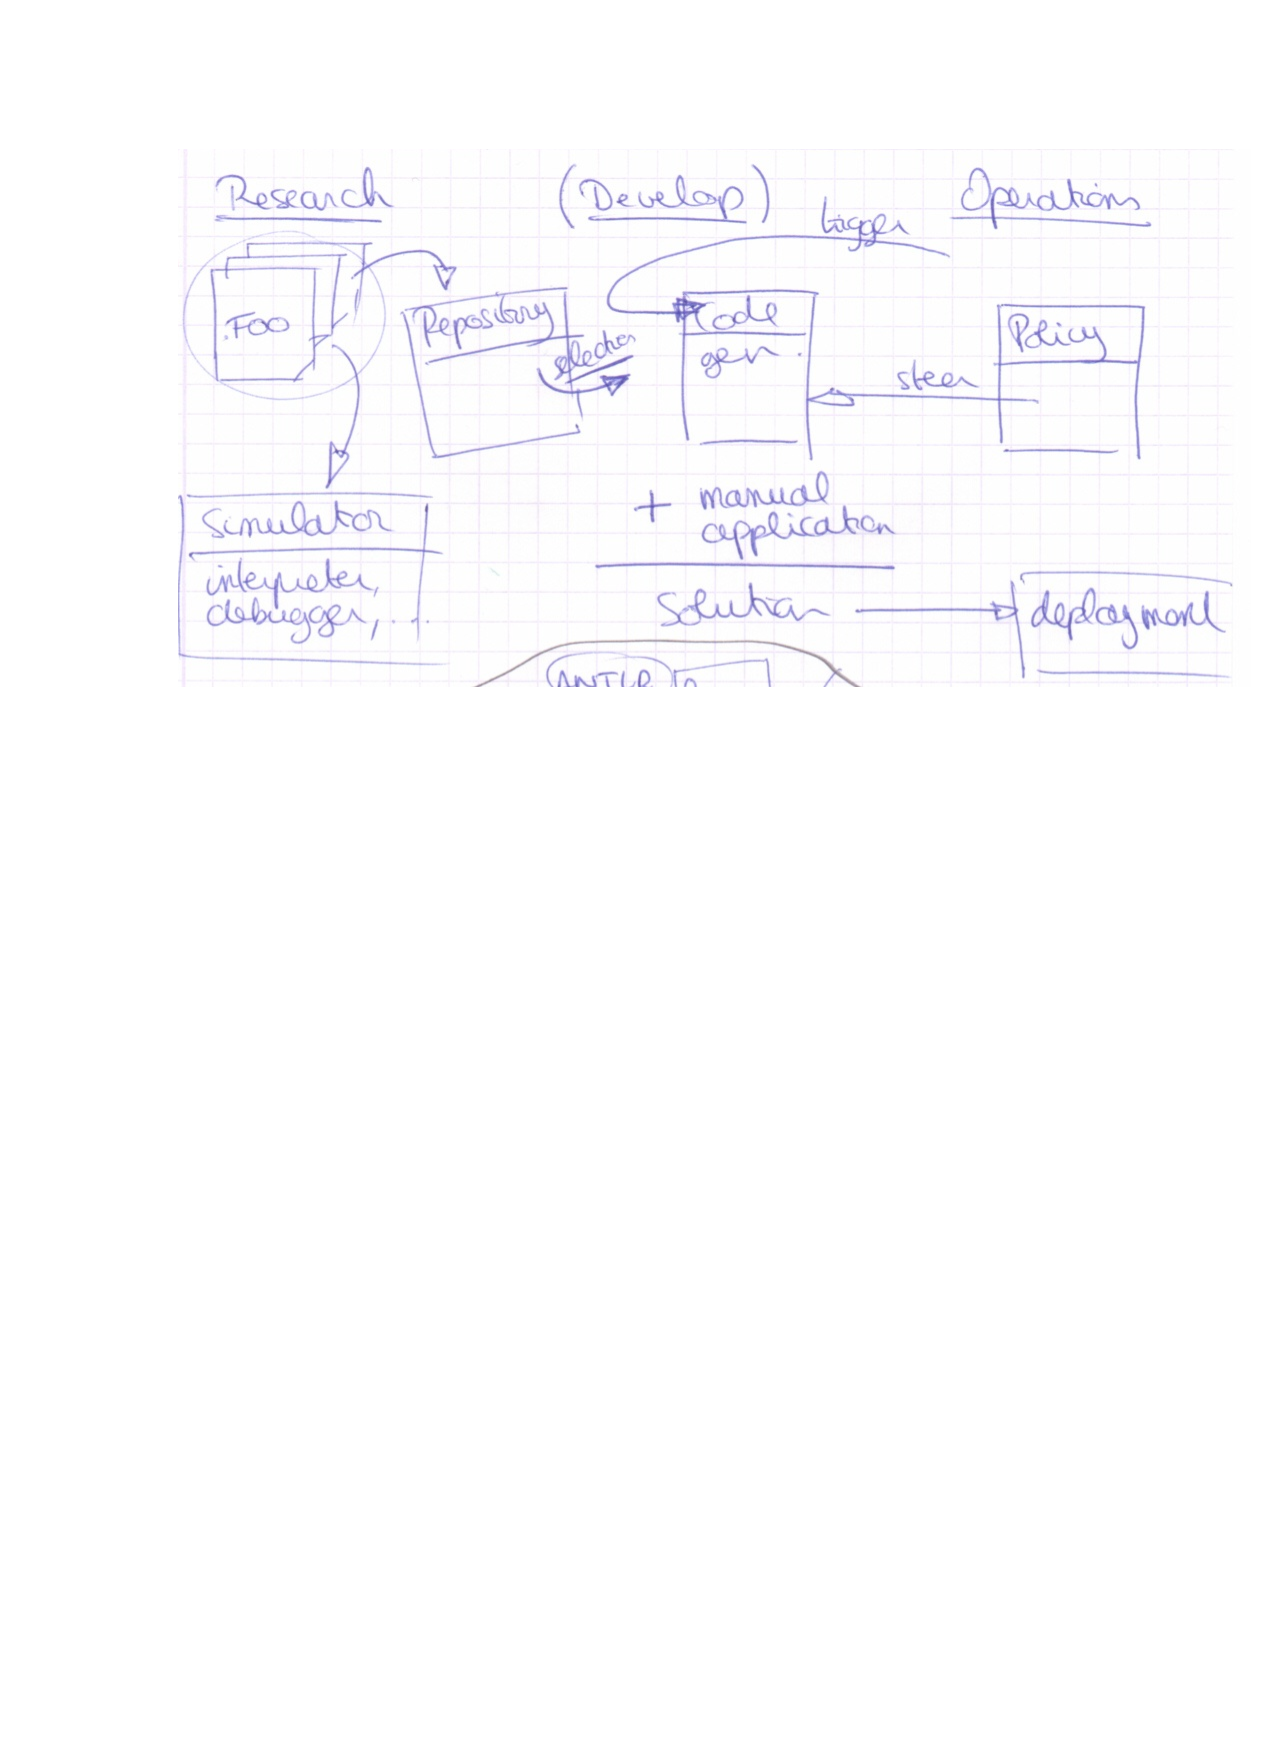
\includegraphics[width=\linewidth]{resources/arch-functional.pdf}
  \caption{Functionele architectuur}
  \label{fig:arch-functional}
\end{figure}

\subsection{FOO-lang}
\label{subsection:arch-foo-lang}

\TODO

\subsection{Centrale opslagplaats}
\label{subsection:arch-repository}

\TODO

\subsection{Code generator}
\label{subsection:arch-codegen}

\TODO

\subsection{Uitbatingsbeleid}
\label{subsection:arch-policy}

\TODO

\subsection{Ontwikkeling en integratie}
\label{subsection:arch-integration}

\TODO

\subsection{Scope}
\label{subsection:arch-scope}

\TODO

\section{Technische architectuur}
\label{section:arch-technical}

\TODO

\begin{figure}[ht]
  \centering
  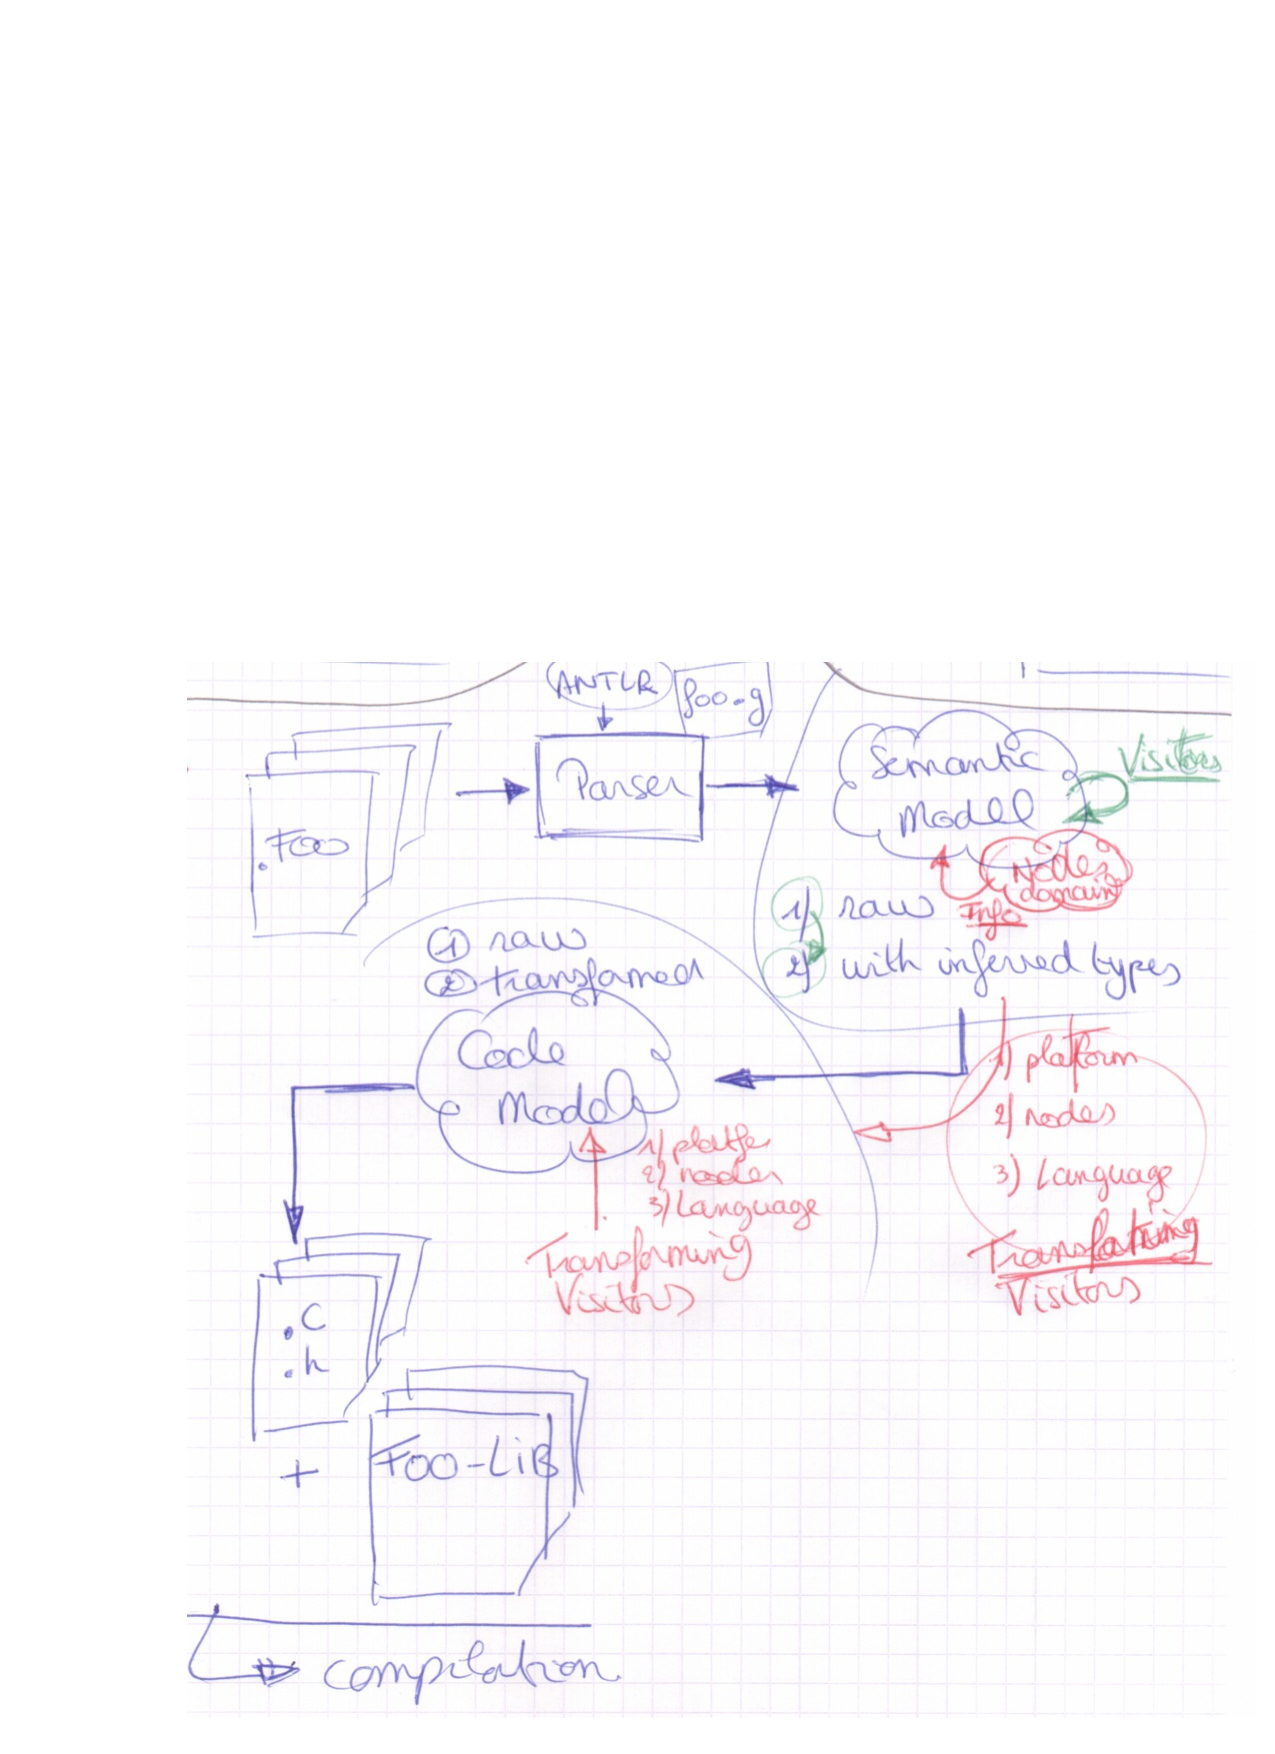
\includegraphics[width=\linewidth]{resources/arch-technical.pdf}
  \caption{Technische architectuur}
  \label{fig:arch-technical}
\end{figure}

\subsection{Semantisch model}
\label{subsection:arch-semantic-model}

\TODO \citep{fowler2010domain}

\subsection{Code model}
\label{subsection:arch-code-model}

\TODO

